\documentclass[10pt]{article}
\usepackage[margin=2cm]{geometry}
\usepackage[T1]{fontenc}
\usepackage{lmodern,graphicx,booktabs,hyperref}
\hypersetup{colorlinks=true,urlcolor=blue}
\hyphenpenalty=10000
\exhyphenpenalty=10000
\emergencystretch=2em
\setlength{\parindent}{0pt}
\setlength{\parskip}{5pt}
\graphicspath{{figures/}}
\begin{document}
\begin{center}
{\LARGE\bfseries Predicting Toronto home prices}\par
{\large SSU Data Dash 2026}\par
Kevin Ryuichi Yamada
\end{center}
\textbf{Repository:} \href{https://github.com/kevinyamada/datadashkevin/tree/model-research-v2}{kevinyamada/datadashkevin, model research branch}\par
\textbf{Draft status:} Video link and final team details must be added before submission.

\section{The problem and the data}
A buyer needs a price estimate before deciding which homes fit their budget. We study two different questions. Without an asking price, how much is the home worth? With an asking price, how much might the listing sell for? We build separate models because asking price contains information that is unavailable for the first question.

The competition supplies 150,000 labelled sales from January 2021 to May 2026. There are two separate files to predict: 3,974 homes without asking prices and 4,064 homes with them. All homes, locations, descriptions and prices are synthetic. Our results therefore do not establish accuracy on real Toronto homes.

Our initial analysis found a median sale price of \$856,650 and a mean of about \$1.07 million. Prices have a long upper tail. About 40.02\% of floor areas are ranges. We use their midpoints and include range information. Lot dimensions are missing for condo apartments, condo townhouses and co ops. This pattern is related to property type, so it should not be treated as random missing data.

We exclude the external valuation estimate and its date. They are absent from both prediction files, and about 70.19\% of their timestamps in the training data occur after the sale. We do not use real maps or census information because the locations are synthetic.

\begin{center}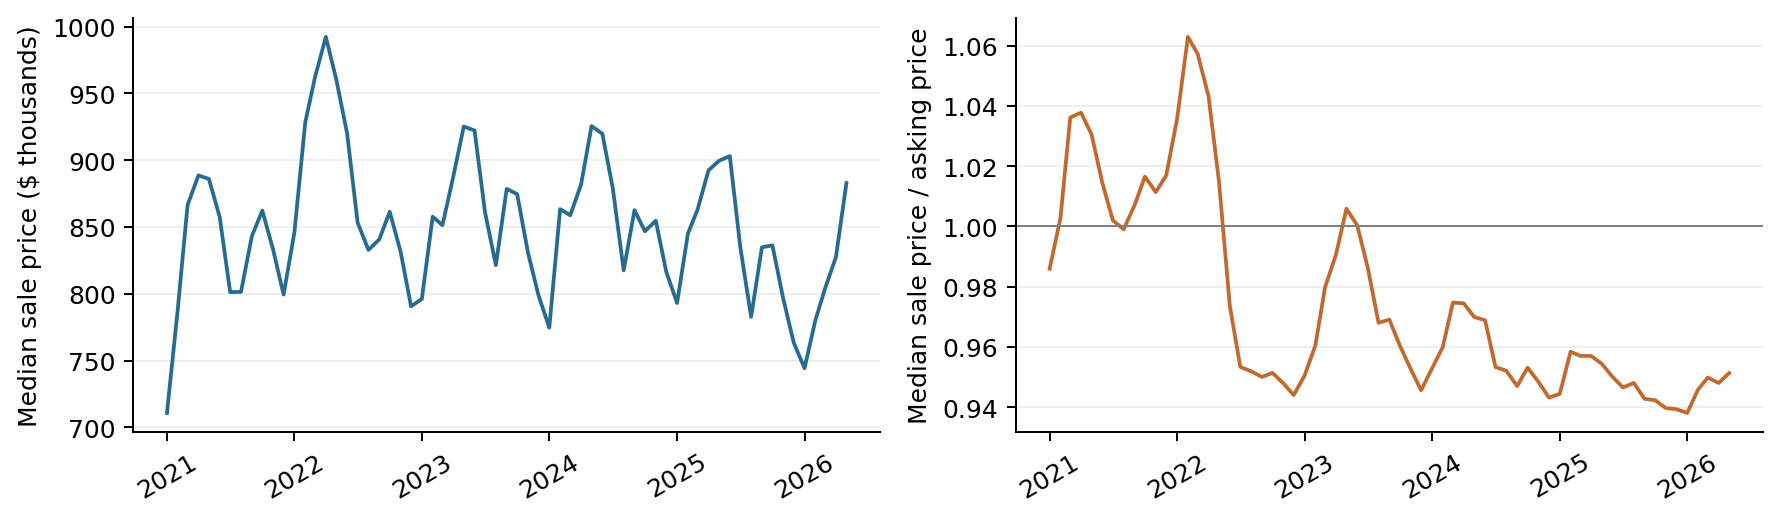
\includegraphics[width=\linewidth]{market.png}\end{center}
{\small Figure 1. Monthly summaries from the labelled data. Changes reflect both market conditions and the types of homes sold. These are descriptive plots, not external market forecasts.}

\textbf{Main result.} On the official monthly validation, median percentage error is 7.44\% without asking price and 4.02\% with asking price. Our previous models scored 9.55\% and 4.11\%. The larger improvement is in the harder task, which carries twice the accuracy weight.

\newpage
\section{Models and fair testing}
\textbf{Without asking price.} We combine LightGBM and spline ridge regression. Both learn log sale price. The final prediction is the geometric mean of their dollar predictions, giving each model equal weight. LightGBM learns interactions between property characteristics. Spline regression fits smoother curves and includes neighbourhood time trends, property type interactions and description text represented by TF IDF.

LightGBM uses squared loss, 1,200 trees, learning rate 0.04, 63 leaves, minimum child size 60 and L2 penalty 5. Its bias correction uses a separate earlier training split: fit before the last three months, predict those three months, then apply half the median log residual as a correction after refitting. No validation outcomes enter that correction. Spline regression uses ridge penalty 10, cubic splines with eight knots and linear extrapolation. The text vocabulary is learned only from the training portion.

\textbf{With asking price.} CatBoost predicts log(sale price / asking price). We convert this back to dollars using the asking price. It uses absolute loss, 1,600 trees, depth 7, learning rate 0.05 and L2 penalty 5. This track uses fixed description flags rather than the spline model's TF IDF representation.

Shared inputs include property type, style, bedrooms, bathrooms, parking, garage, floor area, lot size, synthetic location, listing date terms and description flags. Categories and learned preprocessing are fitted within each training split. Asking price is excluded from the first track. Sale date is used to construct splits, never as a predictor. Days on market, external valuations and the home's own sale price are also excluded from inputs.

\textbf{Model selection.} We screened 35 configurations per track on July to October 2025, trained on earlier sales. We then compared 15 shortlisted fits on November 2024 to February 2025. We assessed individual models and equal weight pairs using their average median error across the two periods. This selected the blend and CatBoost.

\textbf{Supplementary score comparison.} As a supplementary robustness check, we constructed a normalized, weighted norm diagnostic score incorporating MdAPE, MAPE, absolute median signed percentage error, 90th percentile absolute percentage error, and runtime in seconds. Although this score was not used for final model selection, its rankings were broadly consistent with the original mean MdAPE selection criterion. In particular, the selected LightGBM and spline ridge models ranked first and second, respectively, on the confirmation window without asking price, while the selected CatBoost model ranked second with asking price. This agreement suggests that the selected models remained competitive when considering additional predictive performance and computational criteria beyond MdAPE alone. These are rankings of individual models, not a separate evaluation of the blend.

\textbf{Official validation.} For each month from December 2025 to May 2026, we train on sales before that month and predict that month's homes. There are 10,069 predictions per track. Median absolute percentage error is the median of $100|\hat y-y|/y$. Mean absolute percentage error is the mean of the same errors.

\begin{center}
\begin{tabular}{lrr}
\toprule
Model & Median error & Mean error\\
\midrule
Previous model without asking price & 9.55\% & 12.23\%\\
Selected blend without asking price & 7.44\% & 9.87\%\\
Previous model with asking price & 4.11\% & 5.22\%\\
Selected CatBoost with asking price & 4.02\% & 5.09\%\\
\bottomrule
\end{tabular}
\end{center}
These comparisons use our previous fitted models, not the organiser's simple baseline. The organiser's hidden baseline is calculated on the hidden homes.

\textbf{Runtime.} On Windows 11 with Python 3.13.5 and four CPU threads, one fit on all 150,000 labelled sales took 113.45 seconds for the blend and 341.27 seconds for CatBoost. First batch predictions took 1.57 seconds for 3,974 homes and 0.53 seconds for 4,064 homes, respectively. Fit includes preprocessing and internal calibration; data loading and imports are excluded. These are single run timings on one computer, not universal speed claims. The earlier model search took much longer because it repeated training hundreds of times.


\newpage
\section{Price extremes and property types}
The 10th and 90th percentiles of actual validation sale price are \$440,480 and \$1,761,240. Each tail contains 1,007 homes per track; the middle contains 8,055. These groups are retrospective diagnostics, not prediction inputs or rules available before a sale.

\begin{center}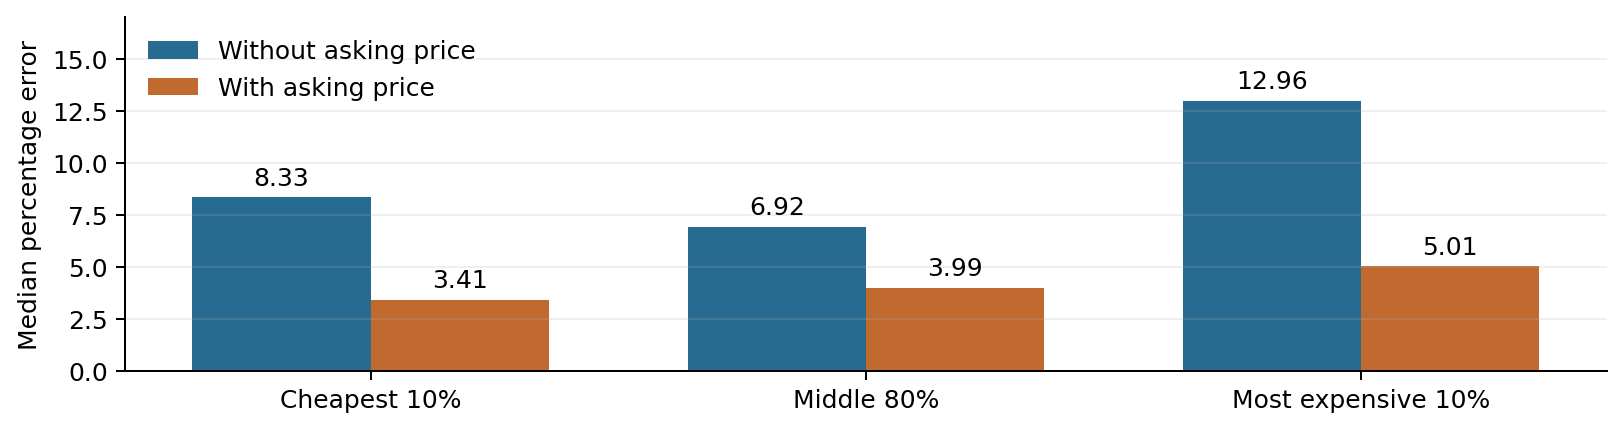
\includegraphics[width=.85\linewidth]{price_extremes.png}\end{center}
{\small Figure 2. Median absolute percentage error by actual sale price. Without asking price, median signed errors are +8.01\% in the cheapest group and $-8.92$\% in the most expensive group, showing overvaluation at the low end and undervaluation at the high end.}

\begin{center}
{\small
\begin{tabular}{llrrr}
\toprule
Price group & Property type & Homes & Without asking & With asking\\
\midrule
Cheapest 10\% & Condo apartment & 975 & 8.32\% & 3.36\%\\
 & Condo townhouse & 18 & 7.05\% & 5.46\%\\
 & Co op apartment & 13 & 13.66\% & 4.48\%\\
 & Detached & 1 & 40.29\% & 8.21\%\\
\midrule
Most expensive 10\% & Detached & 775 & 12.52\% & 5.20\%\\
 & Semi detached & 130 & 12.61\% & 5.62\%\\
 & Freehold townhouse & 52 & 14.62\% & 5.56\%\\
 & Condo apartment & 45 & 32.48\% & 2.69\%\\
 & Co op apartment & 3 & 43.11\% & 3.99\%\\
 & Condo townhouse & 2 & 21.62\% & 7.50\%\\
\bottomrule
\end{tabular}}
\end{center}
{\small Table 2. Median percentage errors within the overall price tails, not within separate type specific tails. Counts are per track. Types with no homes in a tail are omitted. Very small groups, especially those below 30 homes, are descriptive only and should not be used to rank models or property types.}

The cheapest group is mainly condo apartments; the most expensive is mainly detached homes. The 45 expensive condo apartments have much higher error without asking price than detached homes in that tail. This suggests unusual homes need closer review, but does not establish a cause or a reliable future error rate for small groups.

\textbf{Stability checks.} Training once before February 2026 and predicting February to May without refitting gave 7.64\% and 4.14\% median errors. The season differs from the hidden period. A later search of 420 fits found no convincing replacement. A blend with 75\% LightGBM helped older periods but worsened July to October 2025 error from 7.27\% to 7.33\%. Price corrections gave little benefit. We kept the original models and disclose that these periods were reused.

\newpage
\section{Uncertainty, limits and recommendations}
We estimate an interval using absolute log prediction errors from December and January. With $n=2,296$ earlier predictions per track, we take ordered residual number $\lceil0.90(n+1)\rceil$ as $q$. A point prediction $p$ gets the interval $[p e^{-q},p e^q]$. We measure coverage on February to May without using those outcomes to adjust the radius.

\begin{center}
\begin{tabular}{lrr}
\toprule
Track & Monthly refits & No refits for four months\\
\midrule
Without asking price & 90.00\% & 89.81\%\\
With asking price & 87.34\% & 87.30\%\\
\bottomrule
\end{tabular}
\end{center}
The target was 90\%. The second track falls short, so we should not describe those intervals as having demonstrated 90\% coverage. For a hypothetical \$1 million prediction, the ranges are approximately \$811,000 to \$1,233,000 without asking price and \$905,000 to \$1,104,000 with it. They are historical error ranges, not guarantees for a particular home.

An exploratory property based calibration raised coverage with asking price to 92.14\% on reused monthly validation, with wider intervals and a better interval score. It updates using newly observed outcomes, so this does not establish the same benefit for four future months without outcomes. We retain the original intervals and disclose their shortfall.

\textbf{For buyers.} Use estimates to compare homes and plan an initial budget. When an asking price becomes available, use the model designed for that information. Present a range as well as a point estimate. Expensive or unusual homes need closer review.

\textbf{For valuation teams.} Monitor errors by month, property type and neighbourhood. Small groups give uncertain estimates. Review unusual homes rather than applying the average error to every property. A review rule based on predicted price would need its own evaluation; our actual price groups are retrospective.

\textbf{Important limits.} The official months were already seen during earlier work. Our later searches reused historical periods, so none of these results should be called an untouched final test. Some homes were listed before their monthly training cutoff. This follows the starter's sale month convention but does not recreate the information available on every original listing date. We separately checked homes listed after the cutoff; that subset also has a different listing duration mix.

Synthetic descriptions may carry signals that do not transfer to real homes, and a description might not exist before a real listing. Area midpoints are approximate. Tree models and extrapolated spline trends can miss market shifts. Shared market shocks, temporal drift and refitting mean the prediction intervals have no guaranteed future coverage. Hidden sale prices remain unknown.

\textbf{Reproduction.} The sole predictive data source is the \href{https://huggingface.co/datasets/Baliyang/SSU_data_dash}{competition dataset}, pinned to revision \texttt{96a2584}. Run the commands in the repository README. Dependencies, model settings, predictions and experiment summaries are stored with the code. All 34 software tests passed locally; these check software behaviour, not hidden price accuracy. The submission files contain only \texttt{ml\_num} and \texttt{predicted\_price}. The video must be accessible to judges, and the private repository must be shared with organisers before submission.
\end{document}
